\section{Quantitative analysis}\label{sec:quantitative}

We now consider the quantitative implications. We extend the baseline formulation in Section \ref{sec:environment.sec}: First, productivity growth $x_t$ now follows a more general process. This is necessary to capture the empirical patterns of dividend growth. Second, we introduce a force that induces a non-degenerate stationary wealth distribution. A force like this is needed so that belief heterogeneity survives in the ergodic distribution of the model.
We do so through Uzawa endogenous discounting for convenience. This specific approach is not indispensable; we can obtain non-degeneracy through birth-death processes for example.  

\paragraph{Belief process with a continuum of states.}

We start by specifying a continuous Markov process for $x_t$ under both objective and subjective beliefs. 
Let $\hat{x}_{t} \equiv \log x_t $ denote log aggregate productivity growth. Under the objective measure, $\hat{x}_t$ follows:
\begin{equation}\label{eq: x_objective}
    \hat{x}_{t+1} = \mu_x +  \sigma_x \epsilon_{x,t+1}.
\end{equation}
where $\epsilon_{x,t+1} \overset{\text{iid}}{\sim} N(0,1)$. Thus, productivity growth is iid under the objective measure. 

In turn, subjective beliefs about $\hat{x}_t$ for household $i \in \mathcal{I} $ are given by:
\begin{align}
    \hat{x}_{t+1} &= \mu_{x,i} + \rho_{x,i} (\hat{x}_{t} - \mu_{x,i}) + v_{i,t} + \sigma_{x,i} \epsilon_{x,i,t+1},
\end{align}
where $\epsilon_{x,i,t+1} \overset{\text{iid}}{\sim} N(0,1)$. 
Beliefs deviate from the process \eqref{eq: x_objective} in two critical ways:
First, the subjective conditional expectation responds to current productivity growth $\hat{x}_t$. This dimension is important to allow 
households to over- or under-react to past information, consistent with Fact 2 in Section \ref{sec:facts.sec}. Overreaction is controlled by $\rho_{x,i}$. For instance, a positive $\rho_{x,i}$ implies the household overreacts to productivity news, given our assumption that productivity growth is iid under the objective measure. 

Second, beliefs are also exposed to a persistent \textit{sentiment shock} $v_{t}$, which evolve according to
\begin{equation}
    v_{i,t+1} = \rho_{v,i} v_{i,t} + \sigma_{v,i} \epsilon_{v,i,t+1}
\end{equation}
where $\epsilon_{v,i,t+1} \overset{\text{iid}}{\sim} N(0,1)$, and $\epsilon_{v,i,t}$ and $\epsilon_{x,i,t}$ are uncorrelated. 

The sentiment is independent of TFP growth. Thus, this shock leads to fluctuations in the degree of optimism unrelated to fundamentals. Introducing this shock is necessary to quantitatively match the volatility of subjective TFP growth expectations relative to the objective one---Fact 1 in Section \ref{sec:facts.sec}. While extrapolation, through higher values of $\rho_{x,i}$, increases the volatility of subjective expectations, it is insufficient, so the sentiment is needed. 

We note that the belief system in this section is a hybrid of the one in our taxonomy. It encompasses both extrapolation and time-dependent optimism through sentiment shock. We let the survey data discipline the strength of each force. 
% Investors' beliefs deviate from the objective process for $\hat{x}_{t+1}$ in two important ways.
% First, investors disagree about the persistence of states. Some investors believe that positive shocks persist, $\theta_i > 0$, while others believe that shocks revert, $\rho_{x,i} < 0$. 
% Second, beliefs are subject to a common sentiment shock, $v_t$. 
% We impose that the unconditional variance of $\hat{x}_t$ under subjective beliefs coincides with the actual unconditional variance, $Var_i[\hat{x}_t] = \sigma_x^2$. 
% Relative to the objective measure, sentiment shocks cause a larger fraction of the variation of $\hat{x}$ to be attributed to movements in expectations. 
% Sentiment shocks allow us to reproduce the observed volatility of expectations in the data. 
% We further assume that investors agree on the transition probabilities of $w_{t+1}$ and observe its current value. Thus, investors understand that earnings have fat tail. Hence, the only source of disagreement is the persistence of shocks $\theta_i$. 

% Appendix \ref{sec:discretization}  discusses the discretization of the process for $\hat{x}_t$. 
% The discretization provides a state space with dimension $S$  for $x_t$, so $x_t \in \mathcal{X}= \{x^1, x^2, \ldots, x^S\}$,  and transition probabilities $\{p_{ss'}^i\}$, for $s, s' \in \mathcal{S} = \{1,2, \ldots, S\}$. Our discretization implies that the grid $\mathcal{X}$ is the same for all investors, so they agree on the state $s$, but they disagree on the transition probabilities $p_{ss'}^i$.

\paragraph{Endogenous discounting.} 
To ensure the wealth distribution is stationary, we assume that households' subjective discount rate responds to their consumption share:
\begin{equation}
    \beta_{i,t} = \beta e^{\kappa \left(1 - \frac{\mu_i \tilde{C}_{i,t}}{\tilde{Y}_t}\right)}. 
\end{equation}
This assumption, a form of \citet{uzawa2017time} preferences, implies that households' marginal propensity to consume increases with their share of consumption, ensuring that no investor type concentrates all the wealth asymptotically.  Following \citet{schmitt2003closing}, we assume that $\beta_{i,t}$ depends on the average consumption share of type-$i$ households, so households take the process for $\beta_{i,t}$ as given.\footnote{This mechanism is often used in small open-economy models to ensure a stationary distribution of external debt.}

% \paragraph{Model solution.} We describe the model characterization with a continuum of states and Uzawa preferences in Appendix~\ref{app:numerical_solution}. 
% Previous results are essentially unchanged. 
% As in the binary case, an exact closed-form solution is unavailable away from log preferences.
% We compute the solution using a third-order perturbation around the non-stochastic steady state, following, e.g., \citet{van2012term}. 
% A third-order perturbation is indispensable to capture time variation in expected returns.\footnote{For a discussion of the accuracy of the perturbation method, see \citealt{caldara2012computing}.} 
% Simulations are performed using a pruned state-space representation of the higher-order solution to avoid spurious explosive dynamics induced by truncation of the perturbation expansion (see \citealt{andreasen2018pruned}).
\paragraph{Model solution.}
Appendix~\ref{app:numerical_solution} describes the characterization of the model with a continuum of states and Uzawa preferences. The qualitative mechanisms discussed in the binary-state case carry over to this richer environment.
Away from log preferences, no closed-form solution is available. We therefore solve the model using a third-order perturbation around the non-stochastic steady state, following, for example, \citet{van2012term}. A third-order approximation is necessary to generate time variation in risk premia and expected returns.\footnote{For evidence on the accuracy of higher-order perturbation methods, see \citealt{caldara2012computing}.}
Simulations are based on the pruned state-space representation of the higher-order solution (see \citealt{andreasen2018pruned}).


\paragraph{Calibration.} \q{CaliStandardBlock}{We use the following calibration, where parameters are expressed in quarterly terms. Preferences and technology parameters are standard.  \textit{Preferences}: We set $\beta = 0.978$ to match an unconditional annualized risk-free rate of $1\%$. 
The risk aversion is set to $\gamma = 10.0$ and the EIS to $\psi = 2.0$, typical values in the macro-finance literature. 
We choose the labor disutility parameter $\xi$ to normalize the average hours to 1 and set the Frish elasticity to one, $\nu = 1$, a standard value in the literature.
\textit{Technology:} We set $\alpha = 0.66$ and choose $\mu_x$ and $\sigma_x$ to match the average and standard deviation of annual consumption growth of $2.1\%$ and $2.7\%$, respectively.} 

\q{CaliBeliefs}{The calibration of the belief processes is novel. 
\textit{Beliefs:} We focus on the case $I = 2$, and assume that households of type $i = 2$ have rational beliefs, which allows for some rational agents in the environment. We set $\mu_{x,1} = \mu_x$ and $\sigma_{x,1} = \sigma_x$, so households agree on the mean and conditional volatility of productivity growth. 
We set $\mu_2 = 0.1$, so the fraction of rational agents in the population is $10\%$, consistent with the fact that average beliefs in surveys of households and analysts show substantial deviations from rational expectations. 
We set $\rho_{v,1}$ and $\sigma_{v,1}$ to match the persistence of subjective dividend growth and the share of variance explained by movements in expectations, based on estimations of \citet{de_la_o_subjective_2021}.
In turn, we set $\rho_{x,1}$ to match the correlation between subjective expectations and current productivity growth observed in the data. This calibration is agnostic about the relevant belief system: the subjective belief moments pin down these parameters, determining whether non-rational beliefs are extrapolation or rank-preserving. Finally, we set $\kappa = 0.5\%$, consistent with the mean-reversion in consumption shares in \citet{garleanu2015young}.} 

\subsection{Biases in productivity growth expectations}
\label{sec:biases_expectations.sec}
\q{ProdExpectationI}{
In the model, investors hold distorted beliefs about productivity growth.
These distortions propagate to other variables --- such as dividends and returns ---
through the likelihood-ratio representation:
\begin{equation}
    \mathbb{E}_{i,t}[Z_{t+1}]
    =
    \mathbb{E}_t[\ell_{i,t+1} Z_{t+1}],
\end{equation}
where $\ell_{i,t+1}$ is the likelihood-ratio between subjective and objective beliefs.
Hence, a single distortion in productivity growth beliefs induces distortions
in expectations of all equilibrium objects.\footnote{
\citet{cui_subjective_2024} estimate an empirical counterpart to the likelihood ratio
and show that it explains a large fraction of cross-sectional variation in survey expectations.
}

It is therefore important to verify that the model is consistent with the empirical
properties of subjective productivity growth expectations.

\paragraph{Coibion--Gorodnichenko regressions.}

We assess this using Coibion--Gorodnichenko (CG) regressions
\citep{coibion2015information}, which test for systematic forecast biases by regressing
forecast errors on forecast revisions:
\begin{equation}
    \Delta prod_{t+h} - \mathbb{E}_{i,t}[\Delta prod_{t+h}]
    =
    c + \beta_{CG}
    \left(
        \mathbb{E}_{i,t}[\Delta prod_{t+h}]
        -
        \mathbb{E}_{i,t-1}[\Delta prod_{t+h}]
    \right)
    + u_{t+h}.
\end{equation}

Under full-information rational expectations, $\beta_{CG}=0$.
A negative estimate indicates over-extrapolation: agents revise forecasts too strongly
in the direction of recent news.

\paragraph{Empirical implementation.}

As direct survey data on TFP growth expectations are limited, we consider two alternative measures of productivity growth
using quarterly data from the Survey of Professional Forecasters (SPF):
\begin{align}
    \Delta prod^{LP}_{t+1} &= \Delta \hat y_{t+1} - \Delta \hat n_{t+1}, \\
    \Delta prod^{TFP}_{t+1} &= \Delta \hat y_{t+1} - \alpha\,\Delta \hat n_{t+1},
\end{align}
where $\Delta \hat y$ is GDP growth, $\Delta \hat n$ is employment growth, and we set $\alpha=2/3$.

The first measure corresponds to labor productivity growth, and the second is a TFP proxy consistent with how TFP growth is defined in the model.
Table~\ref{tab:cg_productivity_h1} reports the results.
For labor productivity, we estimate
$\hat{\beta}_{CG} = -0.63$,
and for the TFP proxy,
$\hat{\beta}_{CG} = -0.50$,
both statistically significant.

\paragraph{Model comparison.}

We perform the same CG regression using simulated data from the calibrated model.
The model implies
\[
\hat{\beta}_{CG}^{\text{model}} = -0.695.
\]
This value is very close to the empirical estimate for labor productivity
and lies within one standard error of the estimate for the TFP proxy.
}
\begin{table}[!t]
    \centering
    \caption{Coibion--Gorodnichenko Regressions for Productivity Measures}
    \label{tab:cg_productivity_h1}
    \begin{threeparttable}
    \begin{tabular}{lcc}
    \toprule
     & Labor Productivity & TFP Proxy \\
    \midrule
    Forecast revision coefficient $\beta_{CG}$ 
    & -0.63$^{***}$ 
    & -0.50$^{**}$ \\
    & (0.030) & (0.198) \\
    Constant 
    & -0.15 
    & -0.25 \\
    & (0.289) & (0.259) \\
    \midrule
    Observations 
    & 86 & 86 \\
    $R^2$ 
    & 0.3697 & 0.0579 \\
    Adj. $R^2$ 
    & 0.3622 & 0.0467 \\
    \bottomrule
    \end{tabular}
    \begin{tablenotes}[flushleft]
    \footnotesize
    \item Notes: Each column reports OLS estimates of
    $\text{FE}_t = c + \beta \,\text{Revision}_t + u_t$, where $h=1$ quarter.
    Reported standard errors (in parentheses) are Newey--West HAC with lag 4.
    Labor productivity uses $\Delta y - \Delta n$.
    TFP proxy uses $\Delta y - \alpha \Delta n$ with $\alpha=2/3$.
    Sample: 2004Q1--2025Q2.
    Significance: $^{*} p<0.10$, $^{**} p<0.05$, $^{***} p<0.01$ (based on HAC $p$-values).
    \end{tablenotes}
    \end{threeparttable}
    \end{table}

    
    \q{ProdExpectationII}{
    These results support the model's mechanism.
    The same distortions that drive endogenous movements in labor demand
    and risk premia also generate empirically realistic forecast biases
    in productivity growth.
    
    Overall, even though the model is not directly calibrated to productivity-expectations moments, it reproduces the key bias pattern observed in the data.
    }

\subsection{Unconditional moments}\label{sec:unconditional_moments.sec}

Next, we study the model's ability to match unconditional moments. 
To isolate the role of each ingredient, we start from a stripped-down version of the model and progressively add features until we reach the complete model. 
This progression allows us to discuss the role of each ingredient in the model. Table \ref{tab:uncond_moments} presents the results under each formulation.
The table also reports $\pm 2$ standard-error intervals for the data moments.

\q{QuantTable}{
% In preamble:
% \usepackage{booktabs}
% \usepackage{graphicx}

\begin{table}[t]
    \centering
    \caption{Unconditional moments}
    \label{tab:uncond_moments}
    \resizebox{\textwidth}{!}{%
    \renewcommand{\arraystretch}{1.75} % try 1.15-1.3
    \begin{tabular}{@{}lcccccccccccc@{}}
    \toprule\toprule
    & \multicolumn{4}{c}{\textbf{Rational Beliefs}}
    & \multicolumn{6}{c}{\textbf{Subjective Beliefs}}
    & \multicolumn{2}{c}{} \\
    \cmidrule(lr){2-5}\cmidrule(lr){6-11}
    & \multicolumn{2}{c}{\textbf{Endowment}}
    & \multicolumn{2}{c}{\textbf{Production}}
    & \multicolumn{2}{c}{\textbf{Homogeneous}}
    & \multicolumn{2}{c}{\textbf{Heterogeneous}}
    & \multicolumn{2}{c}{\textbf{High elast.}}
    & \multicolumn{2}{c}{\textbf{Data (\(\pm 2\) s.e.)}} \\
    \cmidrule(lr){2-3}\cmidrule(lr){4-5}\cmidrule(lr){6-7}\cmidrule(lr){8-9}\cmidrule(lr){10-11}\cmidrule(lr){12-13}
    \textbf{Variables}
    & \textbf{Mean} & \textbf{Std}
    & \textbf{Mean} & \textbf{Std}
    & \textbf{Mean} & \textbf{Std}
    & \textbf{Mean} & \textbf{Std}
    & \textbf{Mean} & \textbf{Std}
    & \textbf{Mean} & \textbf{Std} \\
    \midrule
    Interest rate           & 10.2 & 0.0 & 10.0 & 0.7 & 10.1 & 1.3 & 1.3 & 6.4 & 1.2 & 6.4 & [0.6, 3.0] & [3.7, 6.0] \\
    Excess returns (equity) &  0.7 & 2.7 & 1.2 & 7.2 & 1.2 & 8.3 & 5.6 &16.8 & 5.7 &16.7 & [3.5, 9.3] & [15.6, 21.4] \\
    \midrule
    Consumption growth      &  2.1 & 2.7 & 2.1 & 2.7 & 2.1 & 2.8 & 2.1 & 2.8 & 2.1 & 3.0 & [1.2, 3.1] & [2.0, 3.4] \\
    Dividend growth         &  2.1 & 2.7 & 2.1 & 9.3 & 2.1 &10.0 & 2.1 &10.0 & 2.1 & 9.8 & [-0.3, 3.4] & [6.9, 11.2] \\
    \midrule
    Log hours               &  0.0 & 0.0 &  0.2 & 0.0 &  0.2 & 1.3 &  0.2 & 1.2 & 0.6 & 1.9 & --  & [1.7, 2.7] \\
    \bottomrule\bottomrule
    \end{tabular}%
    }
    \vspace{0.35em}
    \parbox{\textwidth}{\scriptsize
    \vspace{0.7em}
    \textit{Note:} The table reports annualized unconditional moments in percentage points. Column 1 is the endowment benchmark with rational beliefs; Column 2 adds production with labor chosen in advance under rational beliefs; Column 3 is the homogeneous-beliefs version of the production model; Column 4 is the heterogeneous-beliefs benchmark calibration; Column 5 is the high-labor-elasticity robustness. The data columns report point estimate \(\pm 2\) bootstrap standard errors. Detailed data construction, sample windows, and bootstrap methodology are provided in the Data Appendix (Appendix~\ref{app:data_table5_moments}).
    }
    \end{table}

    
% \begin{table}[t]
% \centering
% \footnotesize
% \setlength{\tabcolsep}{2.5pt}
% \begin{threeparttable}
% \caption{Unconditional moments}
% \label{tab:uncond_moments}

% \begin{tabular}{@{}l*{12}{c}@{}}
% \toprule\toprule
% & \multicolumn{4}{c}{\textbf{Rational Beliefs}}
% & \multicolumn{6}{c}{\textbf{Subjective Beliefs}}
% & \multicolumn{2}{c}{} \\
% \cmidrule(lr){2-5}\cmidrule(lr){6-11}
% & \multicolumn{2}{c}{\textbf{Endowment}}
% & \multicolumn{2}{c}{\textbf{Production}}
% & \multicolumn{2}{c}{\textbf{Homogeneous}}
% & \multicolumn{2}{c}{\textbf{Heterogeneous}}
% & \multicolumn{2}{c}{\textbf{High elast.}}
% & \multicolumn{2}{c}{\textbf{Data}} \\
% \cmidrule(lr){2-3}\cmidrule(lr){4-5}\cmidrule(lr){6-7}\cmidrule(lr){8-9}\cmidrule(lr){10-11}\cmidrule(lr){12-13}
% \textbf{Variables}
% & \multicolumn{1}{c}{\textbf{Mean}} & \multicolumn{1}{c}{\textbf{Std}}
% & \multicolumn{1}{c}{\textbf{Mean}} & \multicolumn{1}{c}{\textbf{Std}}
% & \multicolumn{1}{c}{\textbf{Mean}} & \multicolumn{1}{c}{\textbf{Std}}
% & \multicolumn{1}{c}{\textbf{Mean}} & \multicolumn{1}{c}{\textbf{Std}}
% & \multicolumn{1}{c}{\textbf{Mean}} & \multicolumn{1}{c}{\textbf{Std}}
% & \multicolumn{1}{c}{\textbf{Mean}} & \multicolumn{1}{c}{\textbf{Std}} \\
% \midrule
% Interest rate           & 10.0 & 0.0 & 9.7 & 0.7 & 9.7 & 1.4 & 1.0 & 6.4 & 0.8 & 6.5 & 0.8 & 5.7 \\
% Excess Returns (equity) &  0.9 & 3.0 & 1.4 & 7.9 & 1.5 & 9.3 & 5.8 &17.3 & 6.0 &17.1 & 6.2 &16.5 \\
% \midrule
% Consumption growth      &  1.8 & 3.0 & 1.8 & 3.0 & 1.8 & 3.1 & 1.8 & 3.1 & 1.8 & 3.3 & 1.8 & 3.0 \\
% Dividend growth         &  1.8 & 3.0 & 1.8 &10.3 & 1.8 &11.2 & 1.8 &11.1 & 1.8 &10.9 & \multicolumn{1}{c}{--} &11.5 \\
% \midrule
% Log hours               &  0.0 & 0.0 &-0.1 & 0.0 &-0.1 & 1.5 &-0.1 & 1.3 & 0.0 & 2.1 & \multicolumn{1}{c}{--} & 2.4 \\
% \bottomrule\bottomrule
% \end{tabular}

% \begin{tablenotes}[flushleft]
% \scriptsize
% \item Note: ...
% \end{tablenotes}
% \end{threeparttable}
% \end{table}



% \begin{table}[t!]
% \resizebox{\textwidth}{!}{
% \begin{tabular}{@{}l||ll|ll||ll|ll|ll||ll@{}} \toprule\toprule
%                          & \multicolumn{4}{c||}{\textbf{Rational Beliefs}}                                                         & \multicolumn{6}{c||}{\textbf{Subjective Beliefs}}                    & \multicolumn{2}{c}{} \\
%                          & \multicolumn{2}{c|}{\textbf{Endowment}} & \multicolumn{2}{c||}{\textbf{Production}} & \multicolumn{2}{c|}{\textbf{Homogeneous}} & \multicolumn{2}{c|}{\textbf{Heteregeneous}} & \multicolumn{2}{c||}{\textbf{High elast.}} & \multicolumn{2}{c}{\textbf{Data}}          \\ \midrule
%                          &&&&&&&&&&&\\[-0.7em]
% \textbf{Variables}       & \textbf{Mean}   & \textbf{Std}   & \textbf{Mean}   & \textbf{Std}   & \textbf{Mean}   & \textbf{Std}   & \textbf{Mean}   & \textbf{Std}   & \textbf{Mean}   & \textbf{Std}   & \textbf{Mean}        & \textbf{Std}       \\ 
% &&&&&&&&&&&\\[-0.7em]
% \midrule
% &&&&&&&&&&&\\[-0.7em] 
% Interest rate            & 10.0            & 0.0              & 9.7            & 0.7           & 9.7            & 1.4           & 1.0            & 6.4           & 0.8            & 6.5           & 0.8                 & 5.7               \\
% &&&&&&&&&&&\\[-0.7em]
% Excess Returns (equity)  & 0.9            & 3.0            & 1.4            & 7.9           & 1.5            & 9.3           & 5.8             & 17.3           & 6.0            & 17.1           & 6.2                 & 16.5              \\
% &&&&&&&&&&&\\[-0.7em] \midrule
% &&&&&&&&&&&\\[-0.7em] 
% Consumption growth       & 1.8               & 3.0           & 1.8            & 3.0           & 1.8            & 3.1            & 1.8            & 3.1           & 1.8            & 3.3           & 1.8                 & 3.0               \\
% &&&&&&&&&&&\\[-0.7em]
% Dividend growth          & 1.8               & 3.0           & 1.8            & 10.3           & 1.8            & 11.2           & 1.8            & 11.1           & 1.8            & 10.9            & -                 & 11.5                \\
% &&&&&&&&&&&\\[-0.7em] \midrule
% &&&&&&&&&&&\\[-0.7em] 
% Log hours                & 0.0               & 0.0              & -0.1           & 0.0              & -0.1           & 1.5              & -0.1           & 1.3           & 0.0           & 2.1           & -                & 2.4               \\ \bottomrule\bottomrule
% \end{tabular}}
% \caption{Unconditional moments}\label{tab:uncond_moments}
% \caption*{  \scriptsize 
%     Note: The table reports annualized unconditional moments in percentage points. 
%     Column 1 shows results for the endowment economy limit with rational beliefs. 
%     Column 2 introduces production with the labor friction. 
%     Column 3 shows the case of homogeneous subjective beliefs. 
%     Column 4 presents the case of heterogeneous beliefs with our calibration.
%     Column 5 presents results for an alternative calibration with a higher labor supply elasticity. 
%     The last set of columns shows the corresponding values in the data.
%     Mean and standard deviation of the interest rate and excess equity returns are from \citet{MP85}. Average consumption growth and the volatility of consumption and dividend growth are from \citet{bansal2004risks}. The standard deviation of total hours is obtained from Table 5 in \citet{ohanian2012aggregate}: total hours include changes in employment and hours worked for 1985Q1:2007Q4. Standard deviations in that paper are reported as deviations from an HP-filter. We convert their quarterly figure to annual rates. \par} 
% \end{table}
}

\q{QuantCol1}{
Column 1 presents the stripped-down version of the model with a single representative rational investor, for which hiring is done after TFP is known and labor supply is inelastic. 
This economy behaves as an Epstein-Zin version of the endowment economy studied by \citet{MP85}. The model fails to generate a sizeable equity premium and excess stock volatility. 
Moreover, without the hiring friction, the volatility of consumption and dividends coincide.
Given that rational beliefs are iid, the price-dividend ratio is constant, so return volatility equals dividend volatility.}
% Given the absence of fluctuations in risk premia, there are no labor fluctuations. 

% The first column presents the stripped-down version with a single representative rational investor, for which hiring is done after TFP is known. 
% As explained in Section \ref{sec:environment.sec}, this economy behaves as an Epstein-Zin version of the endowment economy studied by \citet{MP85}.\footnote{We obtain this limit by making $\alpha$ and $\xi$ go to zero, while $\alpha/\xi$ converges to a positive number. In this case, hours equal a positive constant, but wages and labor disutility are equal to zero.} The model fails to generate a sizeable equity premium and excess stock volatility. Moreover, without hiring risk, the volatility of consumption and dividends coincide, and the price-dividend ratio remains constant. Because the price-dividend ratio is constant, dividend growth exactly equals the excess return on equity, leading to constant risk premia and no endogenous labor fluctuations. 


% This seems like a digression -> let's discuss, they are curious about this in letter.
% Near i.i.d. TFP growth plays a critical role in preventing fluctuations in risk premia, hours, and the price-dividend ratio in this classic setting. This is not true away from iid growth, unlike a setting with log preference where the price-dividend ratio is constant regardless of the dividend growth process. Indeed, under log preferences, the price-dividend ratio is constant even though households supply labor: because the labor share is constant, the price and dividends of stocks are proportional to those of human capital. This indicates that, because we are in a setting with a EIS different from 1, i.i.d. dividend growth places limitations to match asset pricing moments and movements in labor. 

\q{QuantCol2}{Column 2 introduces the timing of hires assumption and the elastic labor supply. 
The operating leverage channel endogenously generates differences in volatility between consumption and dividends in line with the data, even though this is not a targeted moment. 
With iid beliefs, there is no time variation in the price of risk, so the model fails to generate fluctuations in hours.
Moreover, the hiring friction implies that dividend growth follows a mean-reverting process.\footnote{
    For models with mean-reverting dividend process, see e.g. \citet{menzly2004understanding} and \citet{santos2006labor}.} 
Without time-varying risk premia, mean-reversion in dividends causes the price-dividend ratio to negatively correlate with realized returns.
This counterfactual behavior dampens return volatility relative to dividend volatility.}

% Column 2 introduces the timing assumption with elastic labor supply. 
% Hiring risk increases the excess return of equity and its volatility. Moreover, this timing enables us to endogenously generate the differences in volatility between consumption and dividend growth observed in the data. This is because the labor share is no longer constant but countercyclical. Quantitatively, the model matches the volatility of dividends, although this was not a target moment. 

% With pre-set labor, the price-dividend ratio is no longer constant. Dividend growth is not iid even though productivity is: periods with higher than expected TFP lead to an increase in dividends, but because TFP growth is iid, on average, dividends are expected to fall after a surprise increase. Movements in the price-dividend ratio are induced by the timing of hires. 
% In fact, even under log, %where the P/E ratio is constant for non-iid dividend processes, 
% the P/E ratio will move. 
% This is because with log, the P/E ratio of the surplus claim is constant, but the returns of human capital and stocks are no longer correlated.   

% While the timing of hires allows the price-dividend ratio to move, it does so in the opposite direction: high TFP periods are associated with high dividends and low prices, leading to pro-cyclical price-dividend ratios. Furthermore, notice that this version of the model cannot generate any movements in hours. This is because even though risk premia increases with the timing assumption---and hours fall on average, risk-premia is not time-varying, given the assumption of rational expectations and iid productivity growth. 

\q{QuantCol3}{Column 3 considers the role of non-rational beliefs calibrated to match the survey data, while abstracting from differences in beliefs. 
In this case, the model does generate movements in hours, given that subjective beliefs are volatile, consistent with the discussion in Section~\ref{sec:analysis.sec4}. 
However, deviations from rational expectations are insufficient to generate an equity premium and stock return volatility in line with the data. 
Movements in subjective beliefs only attenuate the negative correlation between returns and the price-dividend ratio, so return volatility is still dampened relative to dividend volatility.}   
% Column 3 considers the role of non-rational beliefs calibrated to match the survey data, while abstracting from differences in beliefs. In this case, the model does generates movements in hours, given that subjective beliefs are volatile. However, deviations from rational expectations are not enough to generate an equity premium and stock return volatility in line with the data. Furthermore, the direction of movement in the P/E ratio remains problematic. 

\begin{figure}[t!]
    \centering
            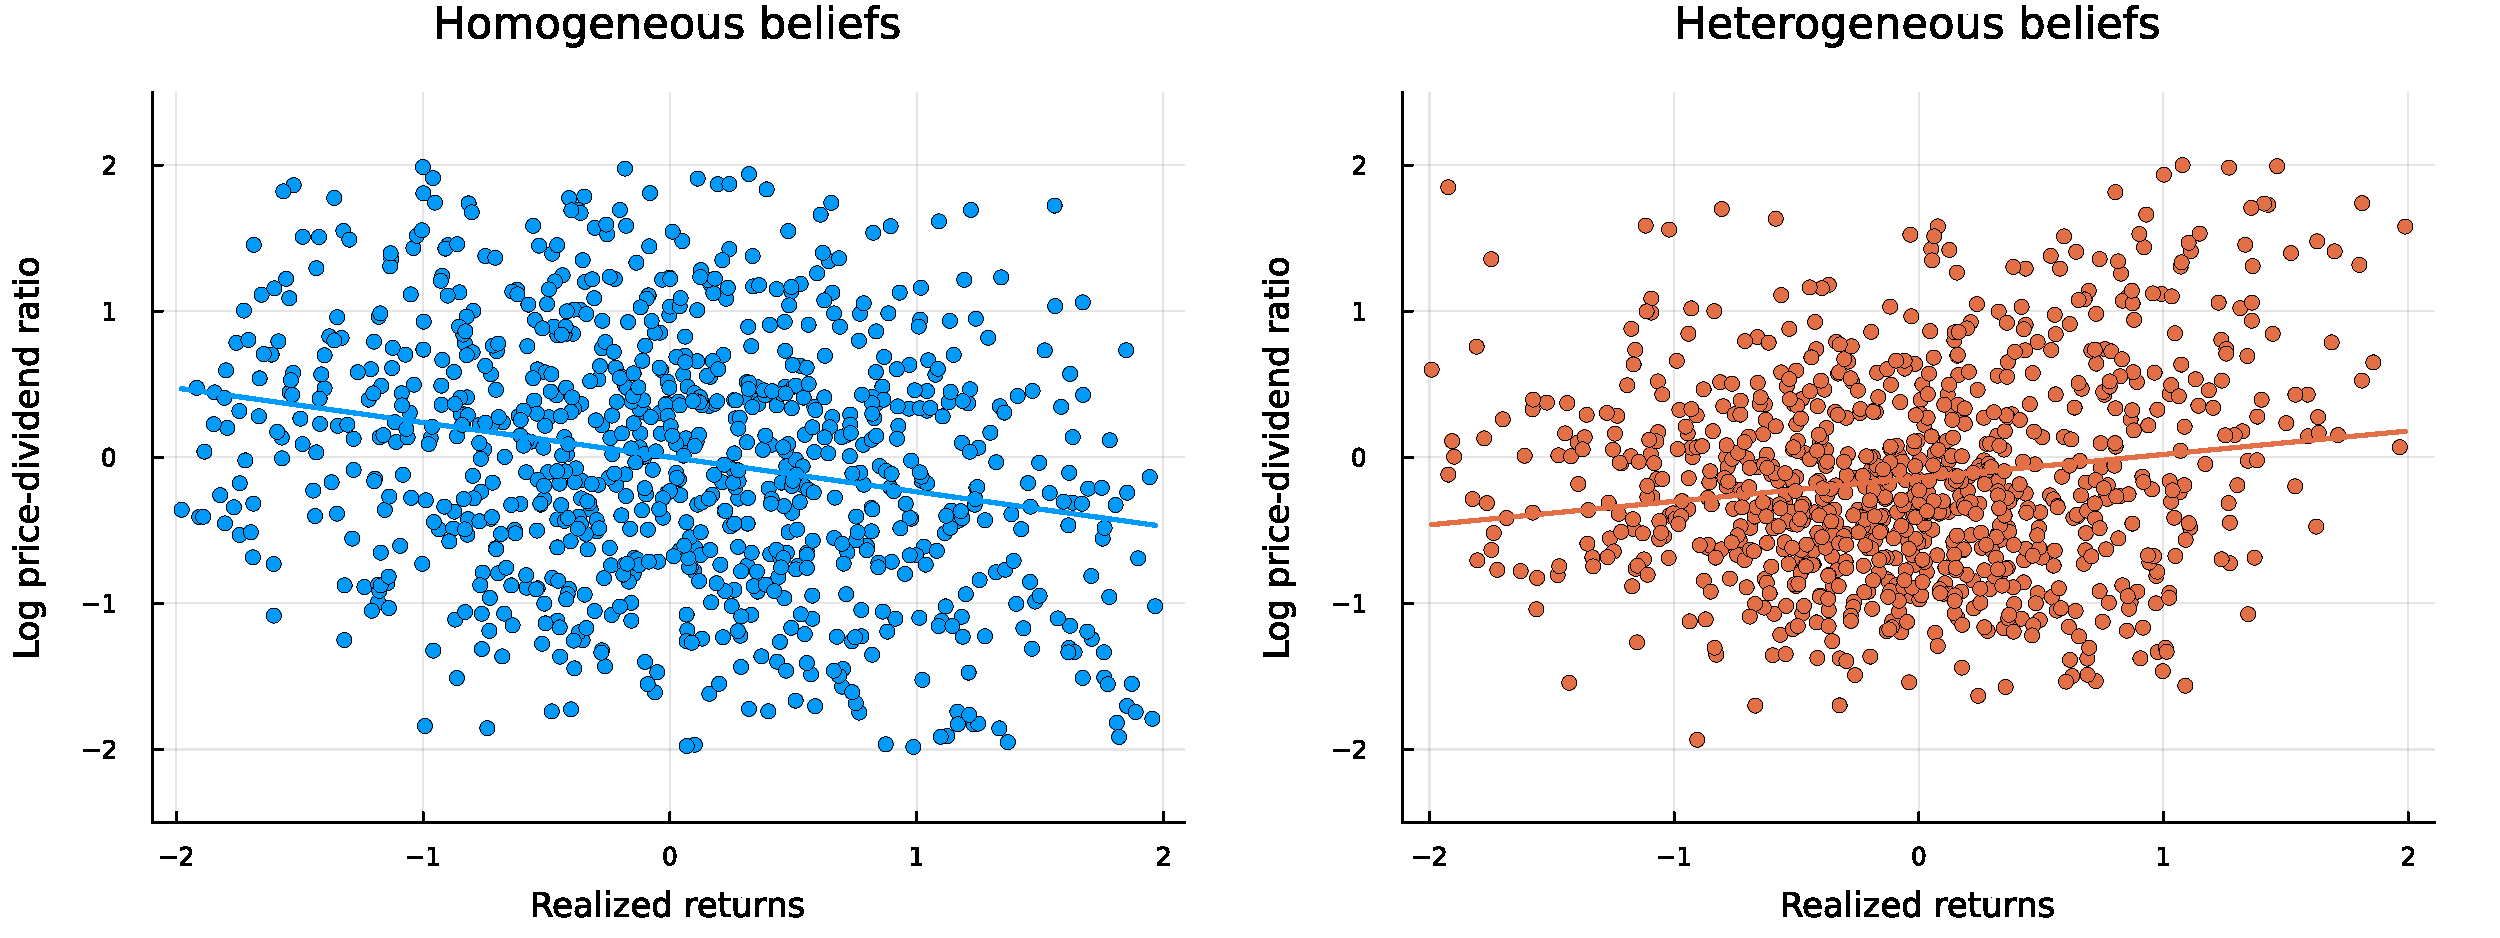
\includegraphics[width=0.99
            \textwidth]{figures/scatter_belief_comparison.pdf}
    \caption{Price amplification: homogeneous vs. heterogeneous beliefs}
    \caption*{  \scriptsize 
    Note: Figure shows a scatterplot of the log price-dividends and realized log returns in a 1,000-period simulation of the model. 
    The left panel shows the simulation for the model with homogeneous beliefs, and the right panel shows the simulation for the model with heterogeneous beliefs. 
    We standardized both variables and removed outliers to improve the visualization.\par} 
    \vspace{0.0cm}
    \label{fig: returns_pd_scatter}
\end{figure}

\q{QuantCol4}{Column 4 introduces heterogeneity in beliefs. 
It brings along rational investors and investors with distorted beliefs. 
The model now generates the level and volatility of asset prices consistent with the evidence, with significant volatility in hours.
To obtain a high equity premium, it is crucial to generate excess volatility of returns. 
This requires the price-dividend ratio to have the right comovement with returns. 
Figure~\ref{fig: returns_pd_scatter} shows that this is the case for the model with heterogeneous beliefs, but not for the model with homogeneous beliefs. 
This success is explained by the time-varying movements in the relative wealth of investors.}

\q{LaborSupplyElasticity}{Column 5 considers an alternative calibration with a higher labor supply elasticity, increasing it from 1.0 to 2.0, the upper limit of the estimates of the macro labor supply elasticity in \citet{keane2012micro}. 
Increasing the labor supply elasticity is motivated by the presence of unmodeled frictions: it is akin to increasing the real wage rigidities. 
While asset-price figures do not change substantially, the volatility of hours almost doubles, aligning the volatility of hours with that of the data.} 

Overall, aside from a modest overprediction of risk-free-rate volatility, the model with heterogeneous beliefs matches key asset-pricing and business-cycle moments.

\q{SV_Extension}{
    \paragraph{Extension with stochastic volatility.}
Appendix~\ref{app:sv_extension} extends the model to allow for stochastic volatility, following \citet{bansal2004risks}. Introducing volatility shocks modestly increases the equity premium and return volatility, while leaving macroeconomic moments largely unchanged. The qualitative conclusions of Table~\ref{tab:uncond_moments} remain intact.
}

\subsection{Excess volatility and return predictability}\label{sec:excess_volatility.sec}

The model's version with heterogeneous beliefs successfully generates empirically relevant levels of excess volatility, i.e., returns that are more volatile than cash flows.
Following \citet{cochrane1992explaining}, we can use a Campbell-Shiller approximation to decompose the variance of the price-dividend ratio into a cash-flow and a discount-rate component:
\begin{equation}\label{eq:var_decomposition}
    Var[pd_t] = Cov\left[ \sum_{k=1}^\infty \rho^k \Delta d_{t+k}, pd_t \right] - Cov\left[ \sum_{k=1}^\infty \rho^k r_{t+k}, pd_t \right],
\end{equation}
where $pd_t$ is the log price-dividend ratio, $\Delta d_{t+1}$ denotes log dividend growth, and $r_{t+1}$ denotes realized log returns.
Expression~\eqref{eq:var_decomposition} connects volatility and predictability. 
It shows that movements in the price-dividend ratio either predict changes in dividend growth or future returns. 
To quantify the relative importance of movements in discount rates, consider the share of variance explained by movements in expected returns, defined as $\beta_{r} \equiv -\frac{Cov\left[ \sum_{k=1}^\infty \rho^k r_{t+k}, pd_t \right]}{Var[pd_t]}$.
As shown, e.g., in \citet{cochrane2011presidential}, empirical evidence suggests that $\beta_{r} \approx 1$, so
discount rates explain most of the price-dividend ratio variance. 

\begin{table}[t!]
    \begin{minipage}[t!]{\textwidth}
      \begin{minipage}[b]{0.5\textwidth}
        \centering 
            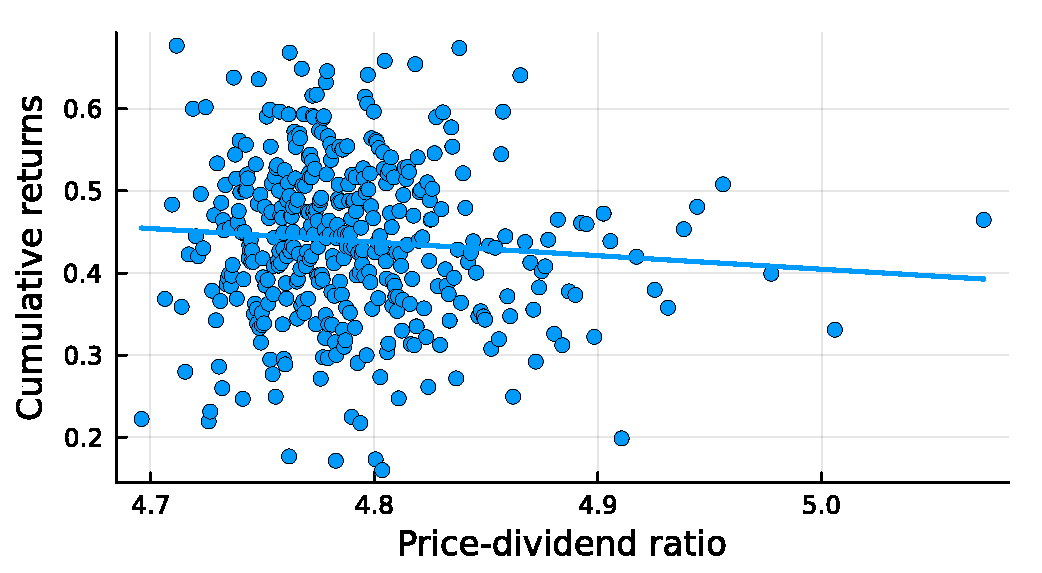
\includegraphics[width=0.99\textwidth]{figures/pd_forecast_binscatter.pdf}
        \captionof{figure}{Return predictability}\label{fig:pd_scatter}
        \end{minipage}
        \hfill
      \begin{minipage}[b]{0.5\textwidth}
        \centering
            \scriptsize
    \begingroup
    \centering\scalebox{0.99}{
    \begin{tabular}{lcccc}
       \tabularnewline \midrule \midrule
       Dependent Variable: & \multicolumn{4}{c}{cum\_ex\_returns}\\
       Model:         & (1)           & (2)            & (3)            & (4)\\  
       \midrule
       \emph{Variables}\\
       labor\_income    &   -2.07   &           & 0.33      &           \\   
                        &   (0.94)  &           & (1.31)    &           \\
       p/d              &           & -0.29     &           & -0.04     \\   
                        &           & (0.12)    &           & (0.17)    \\   
       \midrule
       Observations   & 4,000           & 4,000            & 4,000            & 4,000\\  
       \midrule \midrule
       %\multicolumn{5}{l}{\emph{Heteroskedasticity-robust standard-errors in parentheses}}\\
       \multicolumn{5}{l}{\emph{\textcolor{white}{Signif. Codes: ***: 0.01, **: 0.05, *: 0.1}}}\\
    \end{tabular}}
    \par\endgroup
          \captionof{table}{Labor and p/d ratio regressions}\label{table:pred_regression}
      \end{minipage}
      
      \end{minipage}    
          \caption*{\scriptsize 
        Note: The left panel shows a binscatter plot based on model simulations of the price-dividend ratio and a measure of future cumulative returns, $\sum_{k=1}^T \rho^{k-1} r_{t+k}$, for $T = 60$ quarters. We sort the first 4,000 observations by the price-dividend ratio into 400 equal-count bins and plot bin averages. The right panel shows the regression coefficients of future cumulative excess returns for $T = 60$ on the price-dividend ratio and labor income. 
        The data for the first two columns was simulated under the objective measure, while the data for the last two columns was simulated under subjective beliefs. Entries report Monte Carlo mean coefficients, and parentheses report the standard deviation across simulations.
         }
    \end{table}


    Given that $\beta_r$ corresponds to the slope of a regression of cumulative returns on the price-dividend ratio, the importance of discount rates to explain return volatility is tightly connected to the ability of the price-dividend ratio in predicting future long-run returns. 
    Figure~\ref{fig:pd_scatter} shows that the model with heterogeneous beliefs can capture the predictability patterns observed in the data. 
    The figure shows a strong negative association between the price-dividend ratio and cumulative returns in model-simulated data. 
    Moreover, the coefficient $\beta_r$ in models (4) and (5), as defined in Table~\ref{tab:uncond_moments}, is given by $\beta_r = 0.86$ and $\beta_r = 0.89$, respectively.
    In contrast, we have $\beta_r = -0.15$ for model (2), so the price-dividend ratio predicts returns with the wrong sign, and $\beta_r = 0.26$ for model (3), which has the correct sign but movements in cash flows drive the majority of the fluctuations in the price-dividend ratio. 
    Hence, only versions of the model with belief heterogeneity generate a degree of return predictability that aligns with the data.

    \paragraph{Labor income and return predictability.} 
    \q{OperationalLeverageQuant}{
    Time variation in risk premia generates fluctuations in hours worked in our setting. 
    As a result, in addition to the price-dividend ratio, movements in labor income should also predict excess returns.
    Table~\ref{table:pred_regression} reports the results of a regression of cumulative excess returns on the price-dividend ratio and labor income in our simulated data.
    Column 1 shows that periods of high labor income are associated with lower future returns.
    This finding is consistent with the evidence from \citet{santos2006labor}, who show that a high labor income share predicts lower aggregate stock returns.
    Similarly, \citet{belo2023drives} document that the aggregate hiring rate of publicly traded firms negatively predicts stock market excess returns.\footnote{
        \citet{belo2014labor} and \citet{favilukis2016does} show similar patterns for the cross-section of stock returns and U.S. states.
        For recent evidence using administrative data, see \citet{meeuwis2024time}.
    }    
    Our model links this evidence to fluctuations in subjective beliefs. 
    As discussed in Section~\ref{sec:analysis.sec4}, waves of optimism lead to both an increase in labor income and a compression of risk premia, jointly generating predictability from labor income and the price-dividend ratio. 
    }

    \paragraph{Subjective vs. objective predictability.} 
    The predictability results above are from the perspective of an econometrician. 
    Recent work by \citet{nagel2023dynamics} shows that return predictability looks very different under subjective beliefs: the standard predictors of returns are only weakly associated with survey-based measures of subjective risk premia. 
    While expected excess returns are countercyclical under the objective measure, they appear acyclical under subjective beliefs.
    
    Table~\ref{table:pred_regression} shows that the model replicates these empirical patterns.
    Columns 1 and 2 report predictability regressions using labor income and the price-dividend ratio as predictors under the objective measure. 
    In contrast, Columns 3 and 4 present the same regressions when the model is simulated under subjective beliefs.
    Consistent with \citet{nagel2023dynamics}, standard predictors are only weakly associated with future returns under subjective beliefs. The coefficient on labor income has the wrong sign and is statistically insignificant, while the coefficient on the price-dividend ratio is near zero.
    Thus, our model generates subjective risk premia that are essentially acyclical, which aligns with survey evidence. 
    As discussed in Section~\ref{sec:analysis.sec4}, this acyclicity arises because subjective expectations of future cash flows closely track asset price movements, dampening fluctuations in perceived risk premia.

% \subsection{Return predictability and excess volatility}
% % \paragraph{Connection with classic asset pricing tests.}
% The main postulate of the paper is that differences in beliefs regarding firm earnings growth rates amplify business cycles by affecting firm valuations. Campbell-Shiller, \citep{CampbellShiller88}, offer the following decomposition of the price-dividend ratio:
% \begin{equation}
% pd_{t}=\kappa + \sum^{\infty}_{\tau=0} \rho^{\tau} \mathbb{E}_{t}^{m}[g_{t+\tau}-r_{t+\tau}],
% \end{equation}
% where $pd_{t}$ stands for the log price dividend ratio, $g_{t}$ the growth of dividends and $r_{t+\tau}$ a subjective discount factor. Critically, $\mathbb{E}_{t}^{m}$ is the expectation of the representative market participant. This decomposition is the cornerstone of empirical asset pricing. 

% Because market expectations $\mathbb{E}_{t}^{m}$ are unobservable, we approximate expectations $\mathbb{E}_{t}^{s}[g_{t+\tau}]$ where $\mathbb{E}_{t}^{s}$ is a statistical expectation constructed from econometric models. A challenge put forth by \citet{CochraneDog} is that since aggregate dividends are difficult to forecast with price dividend ratios, the bulk of the movement in stock values must be attributed to changes in discounting. At face value, this conclusion would seem to leave little room for earnings beliefs driving asset prices. However, using $\mathbb{E}_{t}^{s}$ to proxy for $\mathbb{E}_{t}^{m}$, assumes rational expectations. 

% We can recast the Campbell-Shiller decomposition in terms of $\mathbb{E}_{t}^{s}$, $\mathbb{E}_{t}^{i}$ and $\mathbb{E}_{t}^{m}$ to decompose beliefs into deviations from rational expectations and the representativeness of survey data. 
% \begin{align}
% pd_{t}&=\kappa + 
% \overbrace{\sum^{\infty}_{\tau=0} \rho^{\tau} \left[ \mathbb{E}_{t}^{m}[g_{t+\tau}]-\mathbb{E}_{t}^{i}[g_{t+\tau}] \right]}^{\hbox{survey representativeness}}
% +\overbrace{\sum^{\infty}_{\tau=0} \rho^{\tau} \left[\mathbb{E}_{t}^{i}[g_{t+\tau}]-\mathbb{E}_{t}^{s}[g_{t+\tau}]\right]}^{\hbox{belief errors}}
% \\* &+\overbrace{
% \sum^{\infty}_{\tau=0} \rho^{\tau} \left[ \mathbb{E}_{t}^{s}[g_{t+\tau}]
% - \mathbb{E}_{t}^{m}[r_{t+\tau}]\right]}^{\hbox{rational expectations}},
% \end{align}
% Under rational expectations, $\mathbb{E}_{t}^{m}=\mathbb{E}_{t}^{s}$, in which case beliefs do not impact substantially asset prices.
% If beliefs are irrational, $\mathbb{E}_{t}^{m}\not=\mathbb{E}_{t}^{s}$, leaving room for a substantial contribution of beliefs in the volatility of asset prices.  In particular, this contribution will be captured by forecast errors. Let's use this decomposition to see what ingredients of our model are consistent with this classic decomposition.

% \begin{comment}
% \paragraph{Campbell-Shiller Decomposition.}

% The Campbell-Shiller decomposition expresses the log price-dividend ratio as a function of expected future dividend growth and discount rates:
% \begin{equation}
%     p_t - d_t = const. + \sum_{k=1}^T \rho^{k-1} \left[ \Delta d_{t+k}  - r_{t+k}\right] + \rho^T (p_{T} -d_T),
% \end{equation}
% where $\rho$ is a linearization constant. Taking the covariance of this expression with itself, following \citet{cochrane1992}, we obtain:
% \begin{equation}
%     var(p_t - d_t) = cov\left(\sum_{k=1}^T \rho^{k-1} d_{t+k}, p_{t} - d_t \right) - 
%      cov\left(\sum_{k=1}^T \rho^{k-1} r_{t+k}, p_{t} - d_t \right) +\rho^T cov(p_T-d_T,p_t-d_t).\nonumber
% \end{equation}
% \end{comment}

% A variance decomposition of the formula above leads to:
% \begin{equation}
%     1 = \frac{cov\left(\sum_{k=1}^T \rho^{k-1} d_{t+k}, pd_t \right)}{var(pd_t)}
%     -\frac{cov\left(\sum_{k=1}^T \rho^{k-1} r_{t+k}, pd_t \right)}{var(pd_t)} 
%     + \rho^T \frac{cov(pd_T,pd_t)}{var(pd_t)},\nonumber
% \end{equation}
% for large $T$. This equation highlights three possible explanations for variations in the price-dividend ratio: (i) it predicts future dividend growth, (ii) it predicts future returns, or (iii) there exists a rational bubble.

% Empirical evidence, as noted by \citet{cochrane2011presidential}, suggests that the second term is nearly one, meaning that the price-dividend ratio exhibits little predictive power for future dividends, while there is no strong evidence of a rational bubble. This pattern indicates that most of the variation in the price-dividend ratio is driven by fluctuations in discount rates rather than changes in expected future dividends.

% Our model is consistent with this empirical pattern. It generates limited predictability of future cash flows while ensuring that the bulk of price-dividend fluctuations are driven by discount rates. Defining $\omega_{ret}$ as:
% \begin{equation}
%     \omega_{ret} = -\frac{cov\left(\sum_{k=1}^T \rho^{k-1} r_{t+k}, pd_t \right)}{var(pd_t)}
% \end{equation}
% and setting $T = 15 \times 4$ (corresponding to 15 years), we find that $\omega_{ret}$ is approximately one in the data. 

% % \begin{table}[t!]
% % \begin{minipage}[t!]{\textwidth}
% %   \begin{minipage}[b]{0.5\textwidth}
% %     \centering 
% %     	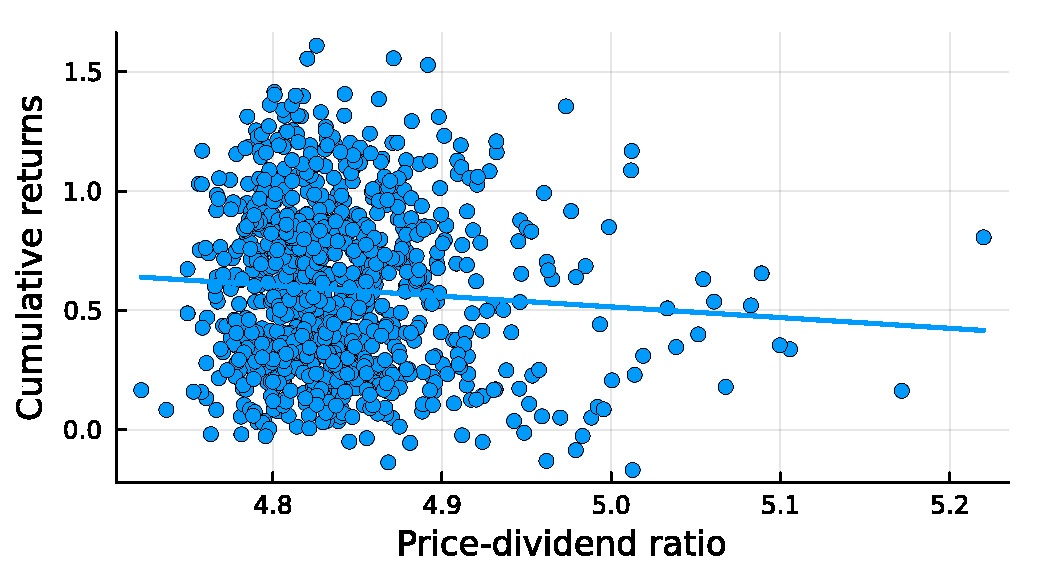
\includegraphics[scale=0.45]{figures/pd_forecast.pdf}
% %     \captionof{figure}{Return predictability}\label{fig:pd_scatter}
% %     \end{minipage}
% %     \hfill
% %   \begin{minipage}[b]{0.5\textwidth}
% %     \centering
% %     	\scriptsize
% % \begingroup
% % \centering\scalebox{0.9}{
% % \begin{tabular}{lcccc}
% %    \tabularnewline \midrule \midrule
% %    Dependent Variable: & \multicolumn{4}{c}{cum\_returns}\\
% %    Model:         & (1)           & (2)            & (3)            & (4)\\  
% %    \midrule
% %    \emph{Variables}\\
% %    p/d    & -0.91       &  & -0.95        & \\   
% %                   & (0.04)      &        & (0.04)       & \\   
% %    labor\_income           &  &   -0.71             & & -0.72\\   
% %                   &      &   (0.19)             &   & (0.20)\\
% %    \midrule
% %    \emph{Fit statistics}\\
% %    Observations   & 4,000           & 4,000            & 4,000            & 4,000\\  
% %    R$^2$          & 0.138       & 0.003        & 0.131        & 0.003\\   
% %    \midrule \midrule
% %    %\multicolumn{5}{l}{\emph{Heteroskedasticity-robust standard-errors in parentheses}}\\
% %    \multicolumn{5}{l}{\emph{\textcolor{white}{Signif. Codes: ***: 0.01, **: 0.05, *: 0.1}}}\\
% % \end{tabular}}
% % \par\endgroup
% %       \captionof{table}{Labor and p/d ratio regressions}\label{table:pred_regression}
% %   \end{minipage}
  
% %   \end{minipage}    
% %   	\caption*{\scriptsize 
% % 	Note: The left panel shows a scatter plot based on model simulations of the price-dividend ratio and a measure of cumulative future returns, $\sum_{k=1}^T \rho^{k-1} r_{t+k}$, for $T = 60$ quarters. The right panel shows the regression coefficients of future cumulative returns for $T = 60$ (first two columns) and $T = 120$ (last two columns) on the price-dividend ratio and labor income. }
% % \end{table}

% This outcome is not mechanical, in the scenario of column (1) where the price-dividend ratio does not vary, $\omega_{ret}$ is undefined. Introducing non-rational beliefs, in column (3), we obtain $\omega_{ret} = -0.16$, which suggests that the model initially dampens return volatility instead of amplifying it, moving in the wrong direction relative to empirical observations. Allowing for richer belief heterogeneity improves the fit, yielding $\omega_{ret} = 0.40$, meaning predictability shifts in the correct direction but still places too much volatility on the cash-flow channel. With further refinements, our preferred specifications reach $\omega_{ret} = 0.93$ and $\omega_{ret} = 0.97$, successfully capturing the empirical finding that most fluctuations in the price-dividend ratio stem from changes in discount rates rather than in expected dividends.
% % , even though the data generating process includes non-rational behavior. 
% This can be seen in Figure~\ref{fig:pd_scatter}, which shows a scatter plot of the price-dividend ratio and future expected returns, as measured by $\sum_{k=1}^T \rho^{k-1} r_{t+k}$. 
% The figure shows how the model with subjective beliefs leads to time-variation in expected returns from the point of view of an econometrician. 


% Importantly, our model avoids the critique raised by \citet{beeler2012long}. 
% Long-run risk models typically predict that the price-dividend ratio should forecast future consumption and dividend growth, a pattern not supported by the data. In contrast, our model does not rely on this channel, sidestepping this issue. Furthermore, our framework aligns well with recent empirical findings by \citet{nagel2023dynamics}, which document that objective discount rates are more cyclical than subjective ones. The model also captures the empirical relationship identified by \citet{santos2006labor}, who provide evidence that labor income predicts future returns.
% Table~\ref{table:pred_regression} shows the result of regressions in simulated data of future cumulative returns on the price-dividend and also labor income. 
% We can see that periods of high labor income predict low future returns, consistent with the connection between labor income and risk premia discussed in Section~\ref{sec:analysis.sec4}. 

% The mechanism underlying these results is straightforward: The model introduces belief heterogeneity, leading to fluctuations in risk premia that impact firm hiring and investment decisions. These movements in discount rates, rather than cash flows, drive asset price fluctuations, aligning our model with the dominant explanation observed in the data. This connection between labor markets, asset prices, and belief heterogeneity provides a unified framework for understanding business cycles and financial markets.












\begin{comment}
\paragraph{Discussion: Beliefs and the Operating Leverage Channel.}

We also know that the labor share would be constant if labor were chosen after productivity was known. Thus, operating leverage, defined as the ratio of revenues minus contemporary variable costs---zero in our setting---to profits would be constant. Yet, there is evidence of xxx correlation, see, e.g., \citet{novy2010operating} and \citet{donangelo2019cross}.\footnote{The relationship between return risk and operating leverage initially appears in \citet{lev1974association}.}. In turn, TFP shocks disproportionately impact dividends relative to consumption; a pattern of more volatile dividends than consumption is consistent with the data  (see, e.g., \citealt{campbell2003consumption}) but inconsistent with models in which hiring is not risky.

%\footnote{This channel is analogous to how changes in the cost of capital, the sum of the interest rate and the firm's risk premium, affects investment decisions.
%The key difference is that the costs and benefits of hiring an additional worker are incurred at the same time, so it is the risk premium, instead of the cost of capital, that affects the hiring decision.
%}
\end{comment}

 
